%*****************************************************
%	APPENDIX
%*****************************************************
\appendix

\chapter{Numerical modeling of polar stochastic processes}
\label{app:modelling}
In this section, modeling techniques for the polar region are explored. Here, the focus is given on developing models for Polar sea ice mechanics and dynamics. An overview of these models is given along with a description of the variables as well as the scope of each model.

\subsubsection{Numerical Modeling of Sea Ice}

The Hibler model is a numerical designed to investigate sea ice dynamics and thermodynamics in the Arctic region \cite{hibler1979dynamic}. This model attempts to couple the sea ice dynamics to Sea ice thickness and uses this relationship to investigate the relationship between the effects of sea ice and the climate. Work so far has largely studied these effects independently using factors that largely ignore the inherent mechanical properties of Sea Ice \cite{hibler1979dynamic}. Coupling these effects would allow for a more general descriptor of Sea Ice spread regions.\par

The model is based off \textcite{coon1974modeling} AIDJEX \cite{hibler1979dynamic}, who use plastic-elastic constitutive laws to describe large-scale sea Ice spreads. It is assumed that cracks, ridges, and leads are randomly distributed on large scales \footnote{100 km from \textcite{coon2007arctic}}. While the Hibler model is not as complex, it is more robust as it allows for larger time-steps and simplifies system boundaries. Here, sea ice is modelled using similar viscous plastic laws \cite{hibler1979dynamic} that allow for non-linear plastic flows to be modelled without severe limitations by large time-steps. The model uses the following components:

\begin{enumerate}
	\item    Momentum balance  - air and water stress
	\item    Coriolis force
	\item    Inertial forces
	\item    Constitutive laws - ice stress, strain, strength
	\item    Ice thickness distribution - accounting for open water patches, changes in thickness and Concentration
	\item    Ice strength 
\end{enumerate}
\begin{equation}
	\frac{mDu}{Dt} = -mfk\times u +\tau_a +\tau_w -mg \nabla H +F 
\end{equation}

$\frac{D}{Dt}$ is the substantial time derivative, k is a unit vector, u is the sea ice velocity, m is the ice mass and f is the Coriolis parameter. Forces in the equation $\tau_a$, $\tau_w$ represent the stress of the air and water respectively where F is the force related to the internal ice stresses. H is the sea surface dynamic height and g is the acceleration due to gravity. Assuming constant turning angles, The air and water momentum equations are as follows
\begin{equation}
	\tau_a = \rho_a C_a|U_g|(U_g cos(\phi)+k\times U_g sin(\phi))
\end{equation}

\begin{equation}
	\tau_w = \rho_w C_w|U_w-u|[(U_w-u)cos(\phi)+k\times(U_w-u)sin(\phi)]
\end{equation}


where $\rho_a $ and $\rho_w$ are the densities of air and water, $C_a$/$C_w$ are the drag coefficients, $U_g$ is the geostrophic wind and $U_w$ is the geostrophic ocean current\par

The Hibler model is the de facto numerical model for large scale ice process \cite{Rutgher2019SmallScale}. The model is used to describe an area of 10 - 100km$^2$, Small scale models are still in development \cite{Rutgher2019SmallScale}.\par 

\subsubsection{Numerical Modeling of Ocean Waves}
Ocean waves are comprised of multiple spectral components with different magnitudes and wave periods knowledge of these spectral components is important for understanding the wave attenuation model \cite{williams2013wave} where, assuming the ice is modelled as a viscous fluid, wave energy is exponentially attenuated \cite{meylan2014situ}\cite{williams2013wave} with distance travelled into the ice due to partial reflections with the ice floes. The rate of attenuation is dependant on the wavelength however an exact mathematical relationship has not been found. The major issue with verifying these models is the lack of robust data availability \cite{meylan2014situ} thereby reaffirming the need for in-situ measurements.\par 
%%% TODO: INCLUDE WILLIAMS WAVE MODELS AND EQUATIONS FOR WAVE SPECTRUM ANALYSIS
\textcite{williams2013wave} describe three fundamental components of Waves in Ice Modeling. These are advection, attenuation, and ice breakage \cite{williams2013wave}. Advection and Attenuation describe how energy transfer occurs between waves and ice and are dependant on the group velocity $c_g$ and the attenuation factor $\hat{\alpha}$ which, in turn, are dependant on the frequency of the wave \cite{williams2013wave}. Also, the properties of ice are significant. These include Young's modulus $Y$, Poisson Ratio $\nu$, strain $\epsilon$ and viscous damping parameter $\Gamma$. The initial Floe Size Distribution and sea ice concentration are also considered. The assumption is that wave breakage feeds back into the model with a new Floe Size distribution \cite{williams2013wave}. \par

Wave advection is described by the following energy model:
\begin{equation}
	\frac{1}{c_g}(\partial_t +c_g\partial_x)S(\omega;x,t) = R_{in}- R_{ice} - R_{other}- R_{nl}
\end{equation}
where $R_{in}$ is the wind input energy, $R_{ice}$,$R_{nl}$,$R_{other}$ represent the energy loss from ice, other sources as well as non linear energy exchanges. $S(\omega;x,t)$ represents the waves in terms of its energy spectral density \cite{williams2013wave} For this model, the energy input is considered to come only from the Rate of exchange between ocean and Ice. Hence all other energy rates are considered 0 and $R_{ice}$ is defined in terms of $\hat{alpha} \text{ and } S$
\begin{equation}
	\frac{1}{c_g}(\partial_t +c_g\partial_x)S(\omega;x,t)  = -\hat{\alpha}(\omega,c,h,\langle D \rangle)S(\omega;x,t)
\end{equation}

$\hat{\alpha} = \frac{\alpha}{\langle D \rangle}$ describes the average attenuation per ice floe. In terms of Ice thickness and wave period \cite{williams2013wave}. By this definition, $R_ice$ is quasi linear \cite{williams2013wave} since a wave with a significantly large Energy spectral density can break the floe decreasing the dimensions $\langle D \rangle$ and increase the dimensional attenuation factor $\hat{\alpha}$. The  operator $(\partial_t +c_g\partial_x)$ serves as the lagrangian reference fram at a moving velocity $c_g$. Finally, by breaking the above model into:
\begin{subequations}
	\begin{align}
		\frac{dx}{dt} = c_g(\omega,t_*,x) \label{advect}\\
		\frac{dS(\omega;x,t)}{dx} = -\hat{\alpha}(\omega,x,t_*,S_*)S(\omega;x,t) \label{atten}
	\end{align}
\end{subequations}

we can describe the dynamics of the sea ice during a breaking event at a time $t_*$ \cite{williams2013wave}. Hence, the model is broken up into an advection model in \ref{advect} and an attenuation model in \ref{atten}.\par

The next step in the model is determining the mathematical model for wave energy. A stochastic approach is taken to define key wave parameters \cite{williams2013wave}. The Significant wave height is found using the formula
\begin{equation}
	H_s = 4\sqrt{m_0[n]}
\end{equation}
$m_n[\eta]$ describes the mean square surface sea elevation of a particle and is derived from the Spectral Density $S$ \cite{williams2013wave}.
\begin{equation}
	m_n[\eta] = \int_{0}{\infty}S(\omega)\omega^nd\omega
\end{equation}

The significant wave height can be considered 4 times the standard deviation of the surface elevation \cite{meylan2014situ}. finally, by determining the significant wave height, the dominant wave period can be calculated as $\frac{1}{f_d}$ where $f_d$ is the frequency at which the dominant wave period occurs \cite{meylan2014situ}.
\subsubsection{Kuik Method}
\label{kuik}
The Kuik method, developed by \textcite{kuik1988method} is a computational technique for measuring and determining the directional characteristics of ocean waves. Measurement of these characteristics are derived from the pitch and roll of an ocean buoy are measured. By using an accelerometer, gyroscope or an inertial measurement system to measure the slope and heave of the 3 axes \cite{kuik1988method}, it is possible to reconstruct the sea state given a set of data provided the data is of a specific length sampled above the Nyquist frequency of dominant ocean swells. A major advantage of the Kuik method is that the parameters are estimated directly from the Fourier transform of the measured signal \cite{kuik1988method} without assumptions about the model. Should the algorithm be used to measure waves in ice, no information is required about the dynamics of the model of the ice floe. This greatly improves the accuracy since ice floes can vary in width, distribution and area as well as change shape due to collisions, freezing and melting. Wind waves are described using a two-dimensional energy spectrum $E$ with wave energy spread over a frequency $f$. The normalised distribution of energy over direction is defined according to \textcite{kuik1988method} as
\begin{equation}
	D_f(\theta) = \frac{E(f,\theta)}{\int_0^{2
			\pi}E(f,\theta)d\theta}
\end{equation} 

Finally, by computing the model per frequency, the distribution simplifies to $D(\theta)$ which can be approximated by a Fourier series with 4 terms \cite{kuik1988method} derived from the pitch, roll and heave of a buoy. Finally, the model can fully characterise the wave spectrum by calculating the following parameters from the Fourier coefficients:

\begin{enumerate}
	\item mean wave direction $\theta_0$
	\item directional width $\sigma$
	\item skewness $\gamma$
	\item kurtosis $\delta$ 
\end{enumerate}

The accuracy of the mean wave direction and width is affected by noise in the sampled data. small RMS values of noise can result in rapid increases of directional width by 1\% to 5\% \cite{kuik1988method}. Additionally, pitch and roll buoys are not free particles. They have an associated mass and therefore an associated inertia \cite{kuik1988method}. This results in a phase shift of the Fourier term by $\phi_i i \in {x,y,z}$  in the first harmonic \cite{kuik1988method}. This shift can result in an error of $0.5^\circ $ for $\sigma > 25 ^\circ $ to $1^\circ \text{ for } \sigma < 10^\circ $ \cite{kuik1988method}   

\subsubsection{Welch-Earle Method}
\label{welchearl}
The Welch-Earle Method is an algorithm for calculating either directional and non-directional wave data depending on the assumptions of the input data \cite{earle1996nondirectional}. Data is derived from the vertical acceleration, roll and pitch of a buoy oriented perpendicular to the surface on either a vertically stabilised platform or a hull-fixed platform \cite{earle1996nondirectional}. Directional wave data is determined from both the acceleration, roll, pitch and heave from the buoy while non-directional wave data is calculated from time-series acceleration only. In this method, a digital time series representation of the vertical Acceleration along with 2 orthogonal Gyroscope measurements and Magnetometer readings relative to the earth’s magnetic field is obtained. The method accounts for the response function of the buoy and provides corrections to phase differences as a result of the buoy's inertia \cite{earle1996nondirectional}. Full directional and non-directional wave data is characterised by calculating the spectra and co-spectra of the time series data. The first part of the method is developed by \textcite{welch1967use} and is used to calculate the power spectral density.
Given a discrete time series data X(j) with a power spectral density P(f), |f|< $\frac{1}{2}$.this data segmented into a set of k-bins $X_k(j) | j \in {0,L-1}$ \cite{welch1967use}. Each bin is multiplied by a selected window function W(k) of length L. Additionally, Bins are taken with a 50\% overlap to produce better statistical averages \cite{earle1996nondirectional} The Fast Fourier Transform (FFT) of the result is taken to for a periodograms $I_k$ \cite{earle1996nondirectional}. Finally, the new power spectral estimator $\hat{P}(f_n)$ is calculated by taking the average of the K periodograms as shown in \textcite{welch1967use}

\begin{equation}
	\hat{P}(f_n) = \frac{1}{K}\sum^K_{k=1}I_k(f_n)
\end{equation}

where 
\begin{equation}
	f_n = \frac{n}{L} | n \in 0,1,2... \frac{L}{2}
\end{equation}

Detrending is used to account for the effects of buoy motion on the time series. The inertia of the platform results in non-zero mean trends often as a result of constant wind or currents acting on the hull of the buoy \cite{earle1996nondirectional}. These must be discarded before the spectrum and co spectra are calculated. The resolution of the accelerometer is important for accurately tracking acceleration \cite{kohout2015device}. If the resolution is too small, low accelerations will not be recorded resulting in incorrect vertical accelerations being calculated. \textcite{kohout2015device} found that a low-resolution IMU was unable to reliably flag that it had exceeded a boundary condition and hence it was discarded \cite{kohout2015device}\par 

The spectra and co-spectra of the directional and non-directional wave series can be calculated by computing the spectrum $S(x)$ as a function of frequency and direction (as is similar to the Kuik method). \textcite{earle1996nondirectional} show that characterisation of the co-spectra $C(x)$ and spectrum$S(x)$ can be achieved by calculating the first 4 Fourier coefficients. Finally, the sea state can be represented by calculating the following parameters

\begin{enumerate}
	\item Longuet-Higgins directional parameters
	\begin{enumerate}
		\item $a_0$
		\item $a_1$
		\item $b_0$
		\item $b_1$
	\end{enumerate}
	\item Significant Wave Height $H_0$
	\item Dominant Wave Period $T_p$
	\item Total Degrees of Freedom $TDF$
	\item Average zero-crossing period $T_{av}$
	\item Zero-crossing period $T_{zero}$
\end{enumerate}

This approach brings into account the possibility of spectral leakage however, this can be greatly minimised by sampling above the Nyquist frequency of the upper Wave frequency band (generally taken to be 0.5Hz) for a minimum of 1000 seconds (about 16 – 17 minutes). Additionally, spectral leakage can be reduced by selecting a window function with a gradual taper such as a half cosine or Hanning taper \cite{welch1967use}\par


\chapter{Mechanical Schematics and Renders}
\label{ch:appendix.schem}

\begin{figure}[H]
    \centering
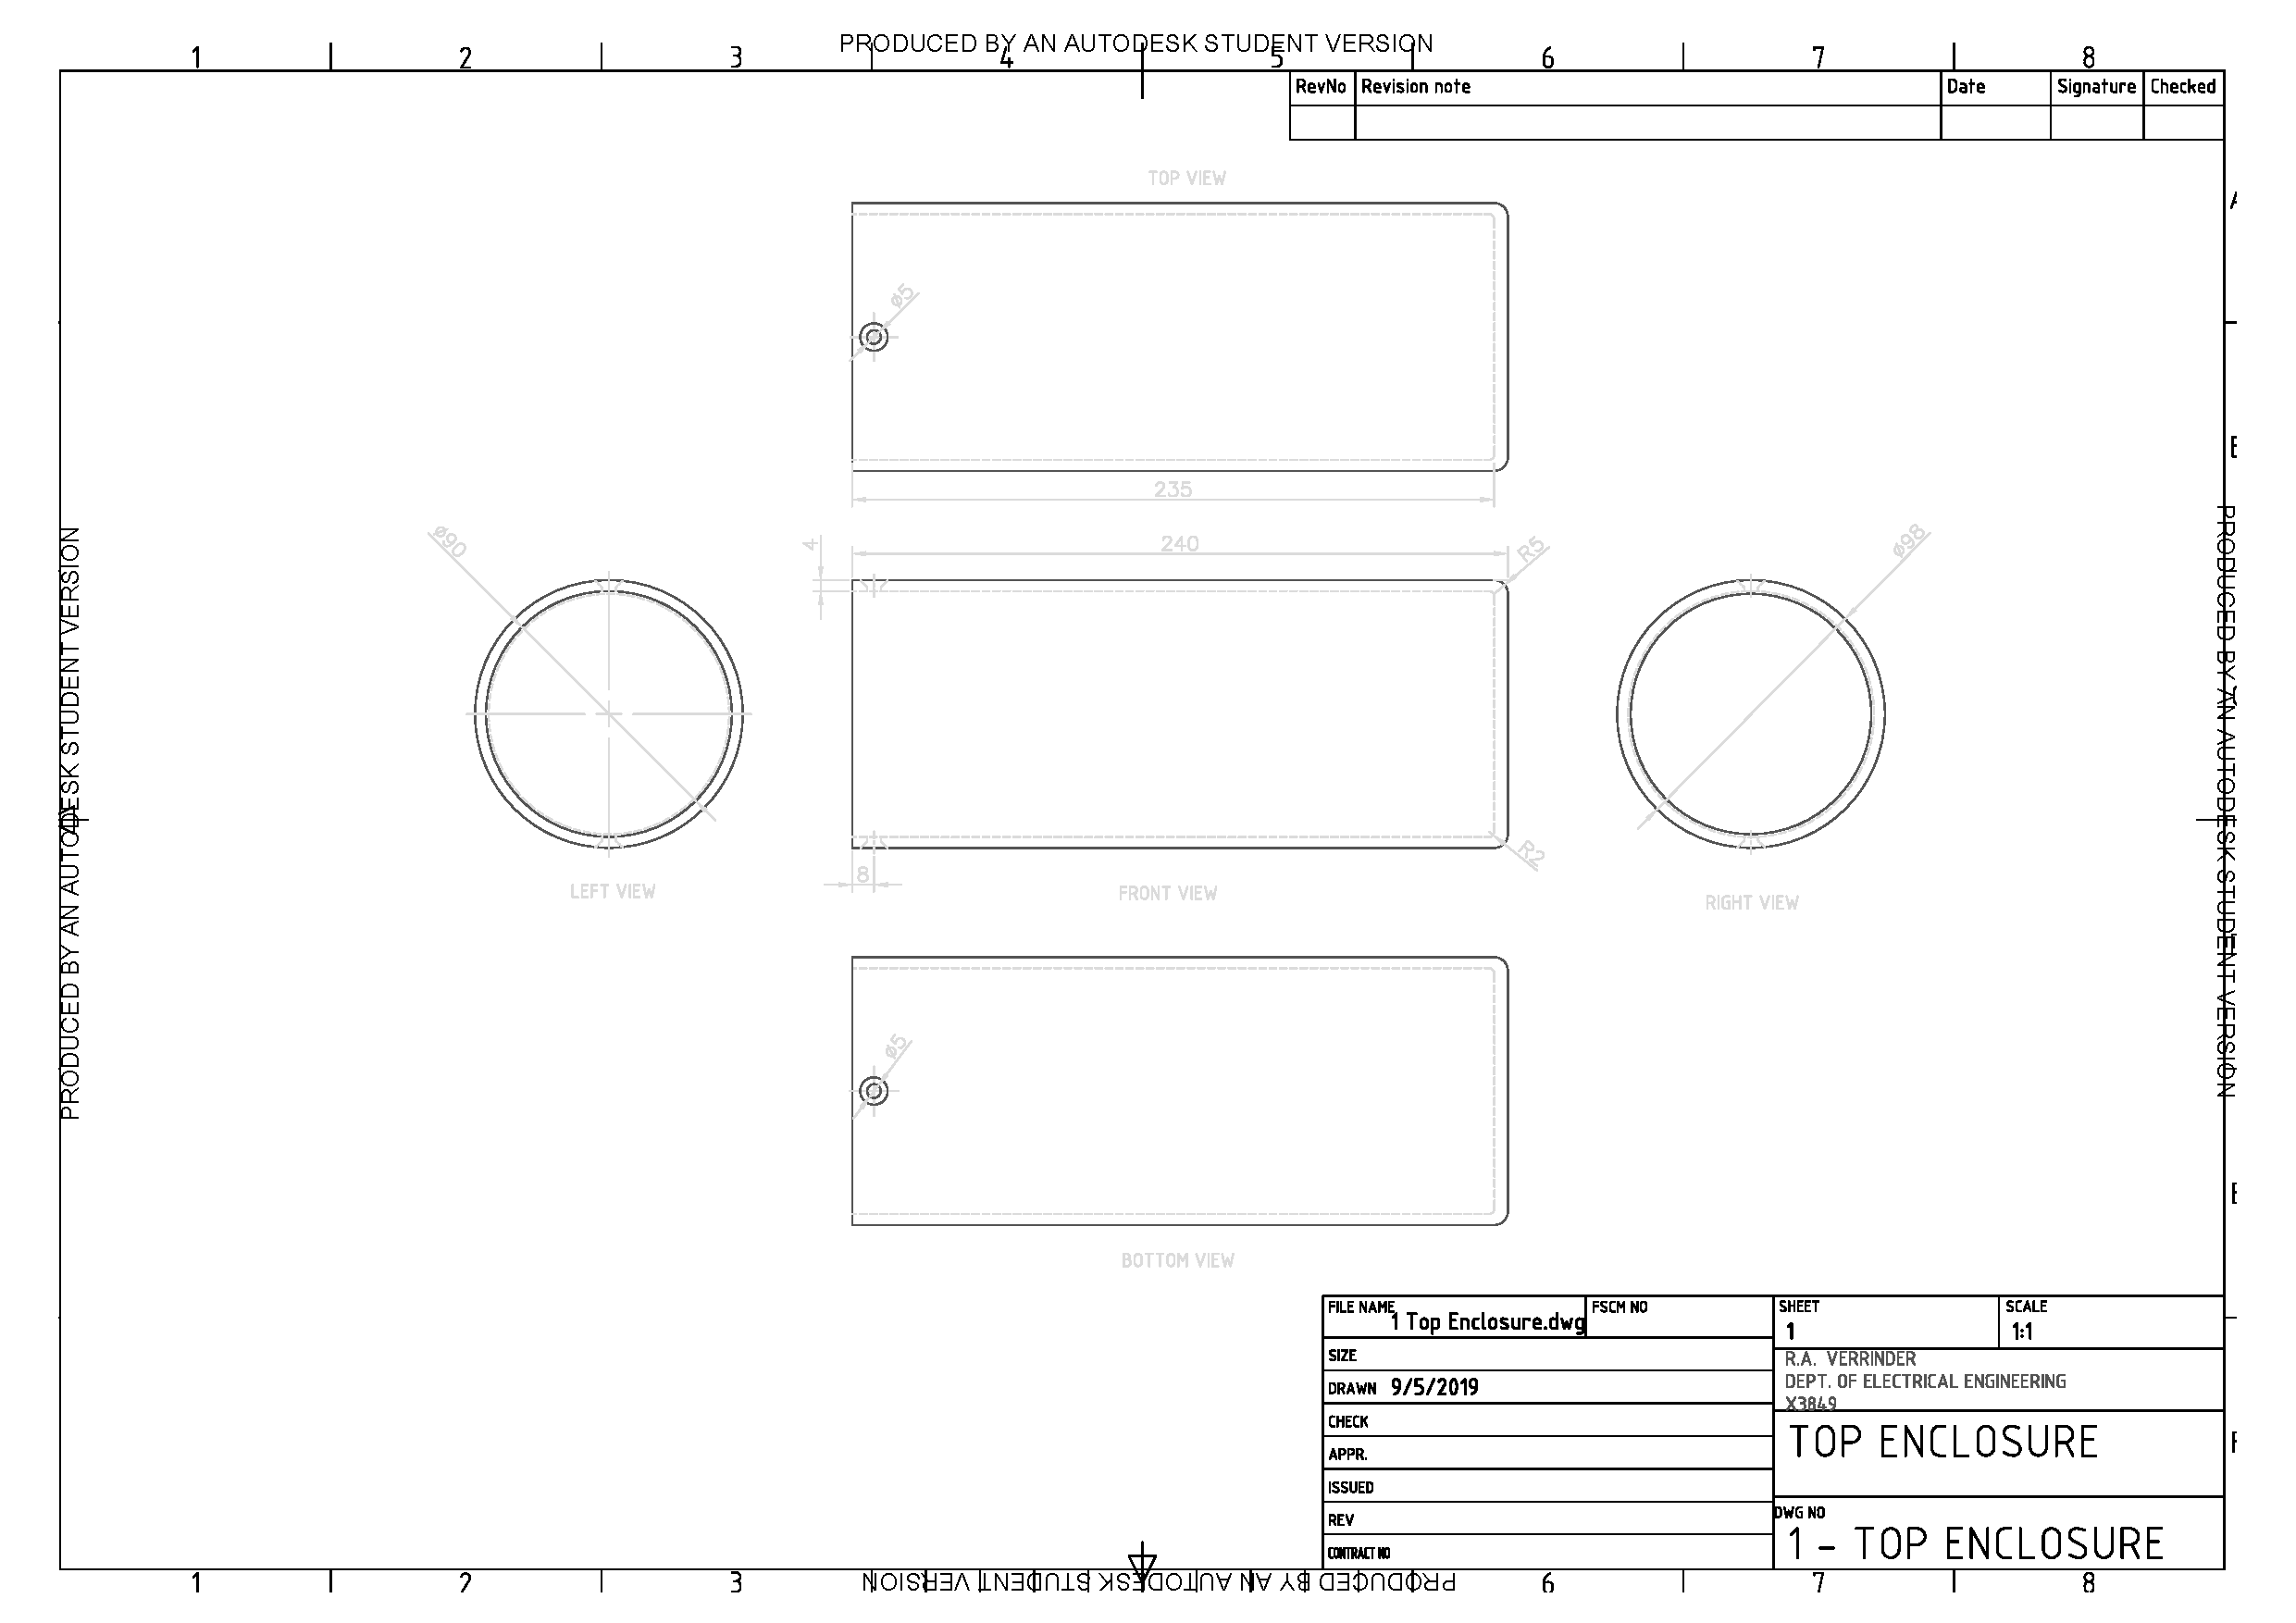
\includegraphics[page= 1,width= 0.9\textwidth]{enclosure}
    \caption{Schematic of Top Enclosure}
    \label{fig:top_schem}
\end{figure}

\begin{figure}[H]
    \centering
\includegraphics[page= 2,width= 0.9\textwidth]{enclosure}
    \caption{Schematic of Bottom Enclosure}
    \label{fig:bot_schem}
\end{figure}

\begin{figure}[H]
    \centering
\includegraphics[page= 3,width= 0.9\textwidth]{enclosure}
    \caption{Schematic of Bottom Enclosure}
    \label{fig:conblock_schem}
\end{figure}

\begin{figure}[H]
    \centering
\includegraphics[page= 4,width= 0.9\textwidth]{enclosure}
    \caption{Full Enclosure Schematic}
    \label{fig:full_schem}
\end{figure}

%Event/ Interrupt description
\chapter{Event and Interrupt Handling protocols} 
\label{sec:evt}

\begin{table}[H]
    \centering
    \caption{Description of Interrupt generated by the iridium module on an external digital input line.}
    \begin{tabular}{|m{0.25\textwidth}|m{0.75\textwidth}|}
    \hline
        \multicolumn{2}{|l|}{\textbf{Ring Indicator}} \\
        \hline
       \textbf{Entry Condition}  &  Buoy In any state other than reset with GPIO mapped to EXTI, with wake up from sleep mode. The WUP Pin receives a Digital High from Ring Indicator Pin on Iridium\\
       \hline
      \textbf{Function} &  The user has transmitted a packet to the buoy. Download the packet and execute/store the data based on the packet structure\\
       \hline
       \textbf{Exit Condition} & Device has downloaded user data which has been used to update the system and store data.\\
       \hline
       \textbf{Return State}& If entry source was a wake up, device will return to sleep. Otherwise device will return to the main loop.\\
       \hline
    \end{tabular}

    \label{tab:Int_desc_RI}
\end{table}

\begin{table}[H]
    \centering
    \caption{Description of routine for interrupts generated by the IMU on an external digital input line.}
    \begin{tabular}{|m{0.25\textwidth}|m{0.75\textwidth}|}
    \hline
        \multicolumn{2}{|l|}{\textbf{IMU Event Detection}} \\
        \hline
       \textbf{Entry Condition}  & Buoy In any state other than reset with GPIO wake up pin mapped to EXTI, with wake up from sleep mode. The WUP Pin receives a Digital High from Interrupt pin\\
       \hline
      \textbf{Function} & Device reads the interrupt source from the IMU, initializes I2C peripheral and begins sampling IMU data. Interrupt source determines the sampling rate, period and mode\\
       \hline
       \textbf{Exit Condition} & Device will exit when the IMU has finished sampling and the data has been stored into memory.\\
       \hline
       \textbf{Return State} & If entry source was a wake up, device will return to sleep. Otherwise device will return to the main loop.\\
       \hline
    \end{tabular}

    \label{tab:Int_desc_IMU}
\end{table}

\begin{table}[H]
    \centering
    \caption{Description of event handling routine for a brown out recovery event.}
    \begin{tabular}{|m{0.25\textwidth}|m{0.75\textwidth}|}
    \hline
    \multicolumn{2}{|l|}{\textbf{Brown out Detection}} \\
    \hline
    \textbf{Entry Condition}  & Buoy is in run mode or in Standby mode with Brown out detection voltage enabled. $V_{brownout}$ has been configured in option bytes. Event occurs when the voltage supplied to the microcontroller is less than $V_{brownout}$  causing the device to be held under reset. When the Voltage rises above the threshold, the device will enter the handler \\
    \hline
    \textbf{Function} & Device resets the relevant register flags and checks for data corruption. If no data is corrupted. Device will reload the last state and attempt to run it again. Otherwise the device performs a software reset \\
    \hline
    \textbf{Exit Condition} & $V_{supply} > V_{brownout}$, device successfully executes code in handler \\
    \hline
    \textbf{Return State} & Returns to main loop\\
    \hline
    \end{tabular}
    \label{tab:Ev_desc_BoD}
\end{table}

\begin{table}[H]
    \centering
    \caption{Description of routine for handling low power events.}
    \begin{tabular}{|m{0.25\textwidth}|m{0.75\textwidth}|}
    \hline
    \multicolumn{2}{|l|}{\textbf{Low Power Detection}} \\
    \hline
    \textbf{Entry Condition}  & Device is in run or sleep, Power Voltage thresholds set in PWR and interrupt enabled. Event occurs when $V_{supply} < V_{power}$ generating an event interrupt. \\
    \hline
    \textbf{Function} & Device will read INA sensor and transmit final packet to base. All peripherals switched off, Device placed into shut down mode.\\
    \hline
    \textbf{Exit Condition} & No Exit\\
    \hline
    \textbf{Return State} & No return state\\
    \hline
    \end{tabular}

    \label{tab:Ev_desc_LPD}
\end{table}

\begin{table}[H]
    \centering
    \caption{Description of routine for handling a software reset event.}
    \begin{tabular}{|m{0.25\textwidth}|m{0.75\textwidth}|}
    \hline
    \multicolumn{2}{|l|}{\textbf{Software Reset}} \\
    \hline
    \textbf{Entry Condition}  & The Microcontrollers NRST internal line is pulled low for a few seconds. This is triggered in any state by triggering a software reset in the NVIC\\
    \hline
    \textbf{Function} & Reset the buoy to an initial state. Clear any pending flags. Reset data in back up registers\\
    \hline
    \textbf{Exit Condition} & Successful reset of voltage domains\\
    \hline
    \textbf{Return State} & Return to Reset state and start of main loop\\
    \hline
    \end{tabular}

    \label{tab:Ev_desc_SWR}
\end{table}


\chapter{Software Figures}

\section{Initialization Routines}

\begin{table}[H]
    \centering
    \caption{Color guide for the initialization routine flow diagrams.}
    \begin{tabular}{l}
    \hline
       \cellcolor{micro}Microcontroller (HAL) function \\
        \cellcolor{sensor}Sensor (API) function \\
        \cellcolor{conditional}Function return statement evaluation \\
        \cellcolor{wrong}Fail return status \\
        \cellcolor{succ}Success return status\\
        \hline
    \end{tabular}

    \label{tab:Init_routine_Guide}
\end{table}


\begin{figure}[H]
    \centering
    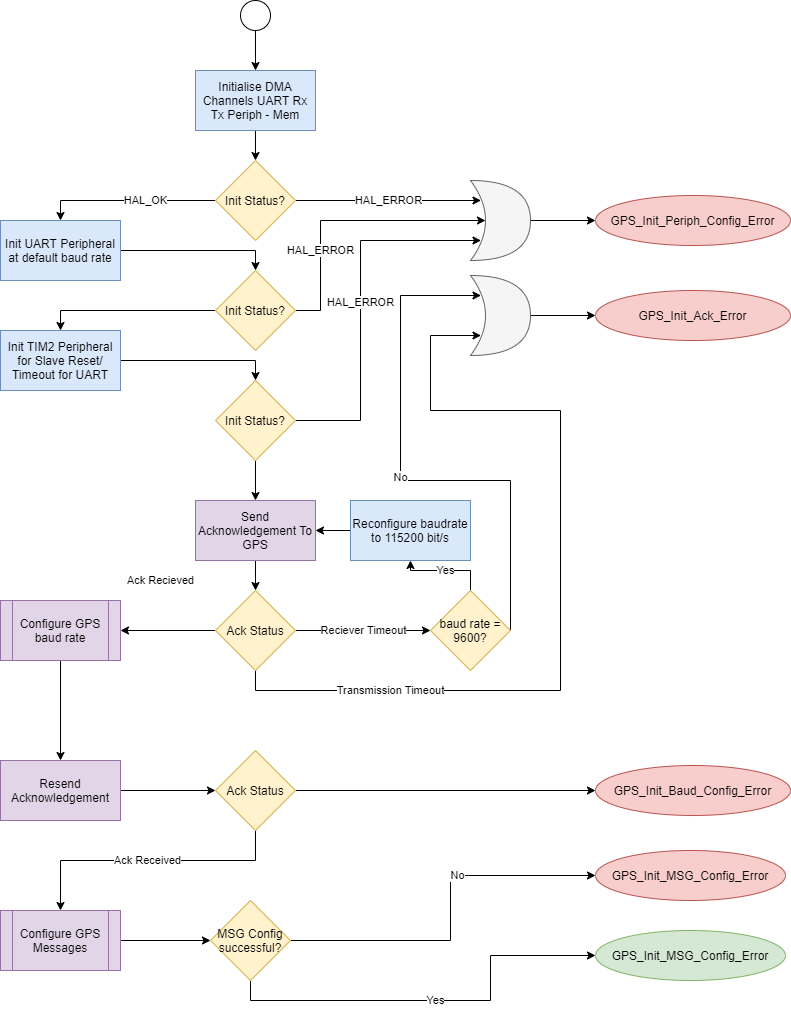
\includegraphics[scale=0.3]{GPS Initialization Algorithm .png}
    \caption{Ublox Neo 7-m initialisation routine}
    \label{fig:Init_diagram_gps}
\end{figure}

\begin{figure}[H]
    \centering
    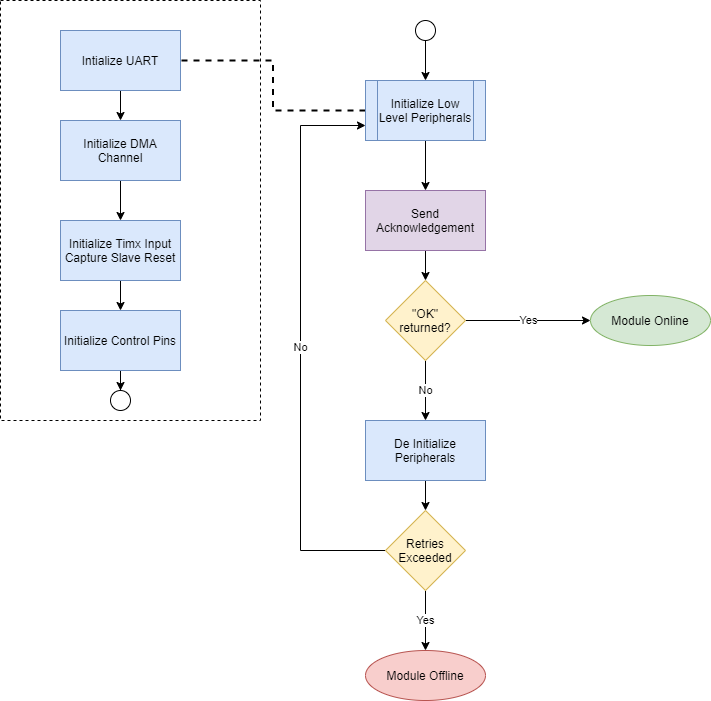
\includegraphics[scale=0.3]{Iridium Init Routine.png}
    \caption{Rockblock 9603 initialisation routine}
    \label{fig:Init_diagram_ir}
\end{figure}


\begin{figure}[H]
    \centering
    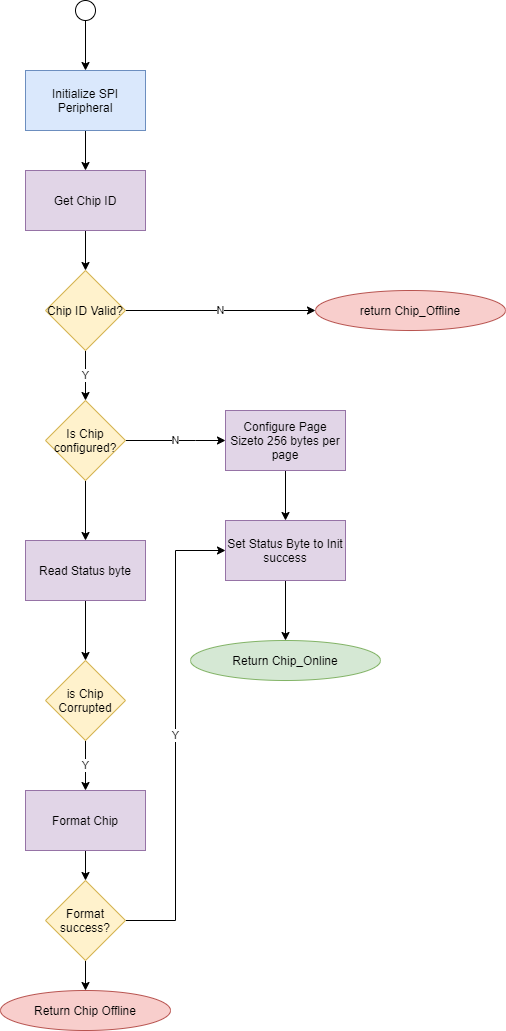
\includegraphics[scale=0.3]{Flash Chip Init Routine.png}
    \caption{AT45DB641E initialisation routine}
    \label{fig:Init_diagram_flash}
\end{figure}

\begin{figure}[H]
    \centering
    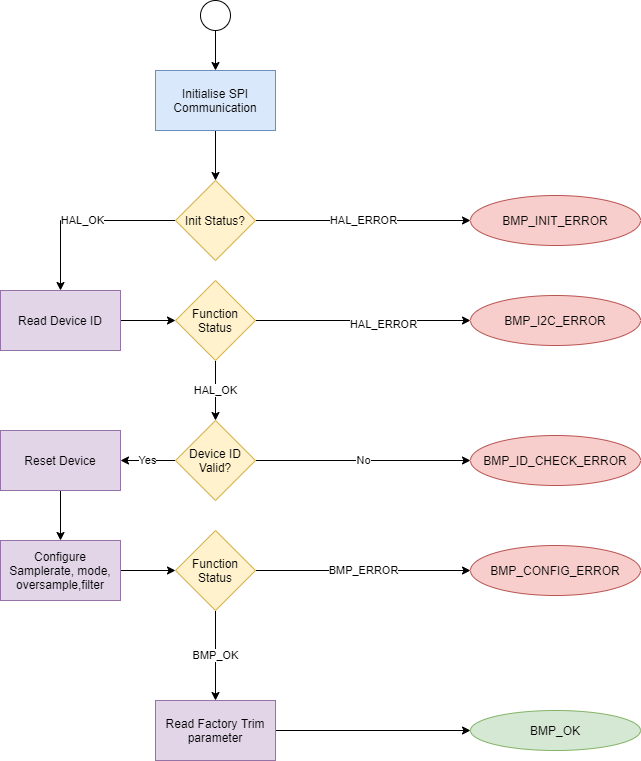
\includegraphics[scale=0.3]{Environmental Sensor Init Routine.png}
    \caption{BMP280 initialisation routine}
    \label{fig:Init_diagram_bmp}
\end{figure}

\begin{figure}[H]
    \centering
    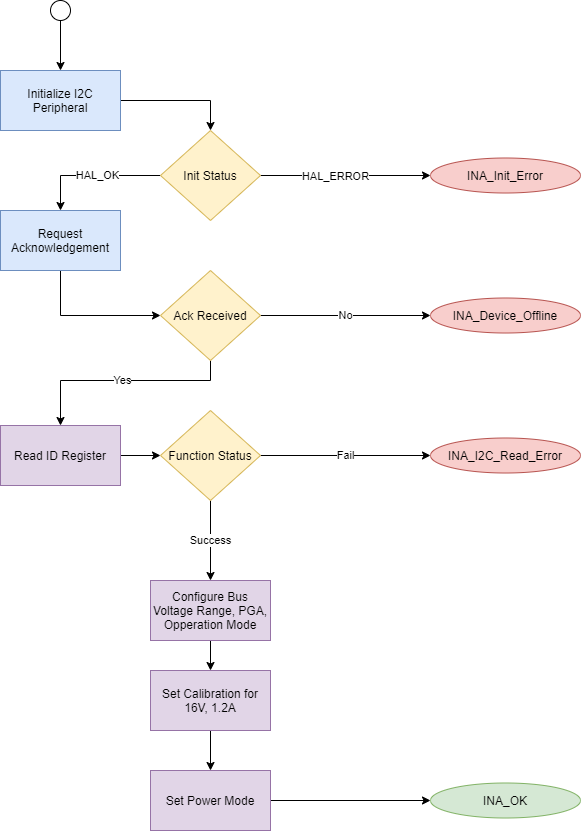
\includegraphics[scale=0.3]{INA219 Init routine.png}
    \caption{INA219 initialisation routine}
    \label{fig:Init_diagram_ina}
\end{figure}

\begin{figure}[H]
    \centering
    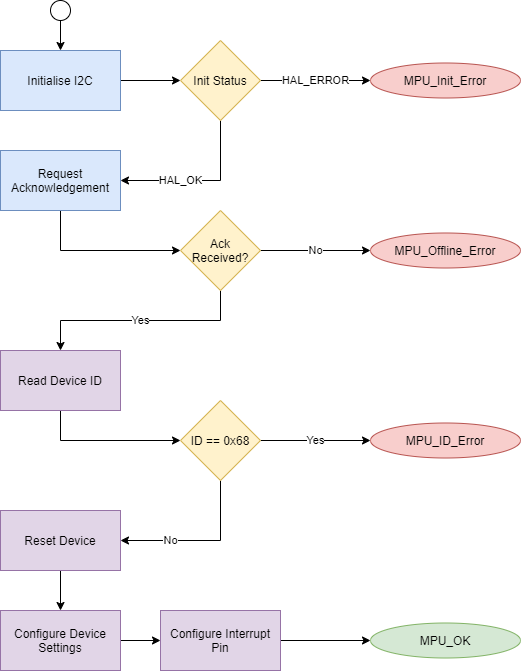
\includegraphics[scale=0.3]{MPU Init Diagram.png}
    \caption{MPU6050 initialization routine}
    \label{fig:Init_diagram_mpu}
\end{figure}

\section{Code}

\subsection{BMP280 Temperature compensation formula}
\begin{figure}[H]

\begin{lstlisting}
/*
 * @brief Temperature Compensation algorithm
 *
 * @param T_val
 * @param t_fine
 * @param bmp_trim
 *
 * @retval int32_t
 */
int32_t BMP280_Compensate_Temp(int32_t T_val,int32_t* t_fine, BMP280_trim_t bmp_trim)
{
	//compensate Temperature from datasheet
	int32_t var1 = (((T_val>>3)- ((int32_t)bmp_trim.dig_T1<<1))*((int32_t)bmp_trim.dig_T2))>>11;
	int32_t var2 =  (((((T_val>>4) - ((int32_t)bmp_trim.dig_T1)) * ((T_val>>4) - ((int32_t)bmp_trim.dig_T1))) >> 12)*((int32_t)bmp_trim.dig_T3)) >> 14;
	int32_t temp = var1+var2; //for storage in global variable
	*t_fine = temp;
	return (temp*5 +128)/256;
}

\end{lstlisting}
    \caption{Function written to compensate  a 32 bit Temperature reading for sensor irregularities using the 32 bit version of the recommended compensation formula from the datasheet \cite{BMP280_Datasheet}. The formula uses the compensation parameters stored on the sensor}
    \label{fig:bmp_code_comp_T}
\end{figure}

\begin{figure}[H]
\begin{lstlisting}
/*
 * @brief Pressure compensation formula
 *
 * @param P_val
 * @param t_fine
 * @param bmp_trim
 *
 * @retval uint32_t
 */
uint32_t BMP280_Compensate_Pressure(uint32_t P_val,int32_t t_fine,BMP280_trim_t bmp_trim)
{
	//Compensation formula
	int32_t var1 = (int64_t)t_fine - 128000;
	int64_t var2 = var1*var1*((int64_t)(bmp_trim.dig_P6));
	var2 = var2 + (((int64_t)bmp_trim.dig_P4)<<35);
	var1 = ((var1 * var1 * (int64_t)bmp_trim.dig_P3)>>8) + ((var1 * (int64_t)bmp_trim.dig_P2)<<12);
	var1 = (((((int64_t)1)<<47)+var1))*((int64_t)bmp_trim.dig_P1)>>33;
	//check for divide by 0 error
	if(var1 == 0)return 0;
	int64_t P = 1048576 - (int32_t)P_val;
	P = (((P<<31)-var2)*3125)/var1;
	var1 = (((int64_t)(bmp_trim.dig_P9)) * (P>>13) * (P>>13)) >> 25;
	var2 = (((int64_t)(bmp_trim.dig_P8)) * P) >> 19;
	P = ((P + var1 + var2) >> 8) + (((int64_t)(bmp_trim.dig_P7))<<4);
	return (uint32_t)P;
}

\end{lstlisting}
    \caption{Function written to compensate  a 32 bit pressure reading for sensor irregularities using the 32 bit version of the recommended compensation formula from the datasheet \cite{BMP280_Datasheet}. The formula uses the compensation parameters stored on the sensor}
    \label{fig:bmp_code_comp_P}
\end{figure}

\subsection{INA219 Calibration Algorithm}
    \begin{lstlisting}[breaklines=true]
/*
 * Function Name INA_Status_t INA219_Calibrate_16V_1_2A(float *I_MBO, float *V_MBO, float *P_Max)
 * @brief: The following function writes a 16 bit value to the calibration register which
 * 			is used to adjust the current, bias voltage and power. Here, A LSB value is
 * 			calculated based on the user requirements and selected from a range. It would
 * 			be advisable to calculate the value manually and replace it in the function below
 * 			please note: the following function has values calculated manually. These can be
 * 			changed based on the configuration settings.
 * 			The values are calculated for 16V bus voltage range with a 2A expected current and
 * 			a 160mV shunt voltage range
 *
 * 	Step 1: V_Bus_Max = 16V
 * 			V_Shunt_Max = 160mV
 * 			R_Shunt = 0.1 Ohm
 *
 * 	Step 2: Max Possible I = 1.6A
 *
 * 	Step 3: Let I Max Expected = 1.2A
 *
 * 	Step 4: Min LSB = 36.6 uA/LSB
 * 			Max LSB = 292.97 uA
 *
 * 			Choose LSB = 100 uA
 * 	Step 5: Set Calibration value = 4096
 */

INA_Status_t INA219_Calibrate_16V_1_2A(float *I_MBO, float *V_MBO, float *P_Max)
{
	//set Current Step Size
	ina.INA219_I_LSB = 100.0/1000000.0;
	uint16_t I_cal_val = (uint16_t)(0.04096/(ina.INA219_I_LSB*INA219_R_SHUNT));
	ina.INA219_P_LSB = 20*ina.INA219_I_LSB;
	float I_max = ina.INA219_I_LSB*32767;
	if(I_max  > 1.6) //max possible current
	{
		*I_MBO = 1.6;
	}else
	{
		*I_MBO = I_max;
	}
	float Vshunt_max = *I_MBO*INA219_R_SHUNT;
	if(Vshunt_max > 0.16)
	{
		*V_MBO = 0.16;
	}
	else
	{
		*V_MBO = Vshunt_max;
	}
	*P_Max = *I_MBO*16;

	//write I_Cal_val to register
	uint8_t temp[2] = {(I_cal_val&0xFF00)>>8,(I_cal_val&0x00FF)};
	if(HAL_I2C_Mem_Write(&ina.ina_i2c,INA219_I2C_Address,CALIBRATION_REG,1,temp,2,100) != HAL_OK)
	{
		return INA_I2C_WRITE_ERROR;
	}

	return INA_OK;
}

\end{lstlisting}
\begin{center}
\captionsetup{type=figure}
\captionof{figure}{Calibration routine for INA219 Current sensor for a maximum current of 1.2A, maximum Bus Voltage of 16V and maximum shunt voltage of 160mV}
\label{fig:INA_Calib}
\end{center}

\subsection{Data Structs}
\begin{figure}[H]
    \centering
\begin{lstlisting}
/*
 * Coordinate Object
 *
 * Stores the Cordinates of GPS in the form DDMM.mmmm
 * where 
 *          DD     -   Degrees
 *          MM     -   Minutes
 *          mmmm   -   Fractional minutes
 * Variables:	Name.............Type.................................Description
 * 				lat..............float32_t............................GPS Lattitude
 * 				longi............float32_t............................GPS Longitude
 */
typedef struct
{
	float_t lat;
	float_t longi;
}Coord_t;
\end{lstlisting}    
    \caption{Coord\_t Data structure to store incoming GPS coordinates as IEEE754 32-bit floats}
    \label{fig:data_coord_t}
\end{figure}

\begin{figure}[H]
    \centering
\begin{lstlisting}
/*
 * Diagnostic Object
 *
 * Structure to Hold the GPS data signal diagnostics
 *
 * Variables:	Name.............Type.................................Description
 * 				PDOP.............DOP_t................................Positional Dilation of Precision (3D)
 * 				HDOP.............DOP_t................................Horizontal Dilation of Precision
 * 				VDOP.............DOP_t................................Vertical   Dilation of Precision
 * 				num_sats.........uint8_t..............................Number of Satelites used to obtain positional Fix
 * 				fix_type.........uint8_t..............................number between 1-3 describing the type of fix obtained
 *
 * Fix types
 * 1 - No Fix
 * 2 - 2D Fix (No altitude)
 * 3 - 3D Fix
 */

typedef struct
{
	DOP_t PDOP;
	DOP_t HDOP;
	DOP_t VDOP;
	uint8_t num_sats;
	uint8_t fix_type;
}Diagnostic_t;
\end{lstlisting}
    \caption{Data Structure for storing GPS signal diagnostic information}
    \label{fig:data_Diagnostic_t}
\end{figure}


\chapter{Supplementary Tables}

\begin{table}[H]
    \centering
    \caption{ List of data services provided by Iridium for transmission of data over the satellite network including the bandwidth and purpose of the service taken from \cite{iridium_mobile}}
    \label{tab:iridium service}
     \vspace{2.5mm}
    \begin{tabular}{|>{\RaggedRight}m{0.2\textwidth}|>{\RaggedRight}m{0.25\textwidth}| >{\RaggedRight}m{0.2\textwidth}| >{\RaggedRight}m{0.3\textwidth}|}
    \hline
    \textbf{Service Name} & \textbf{Purpose}& \textbf{Supporting Modems} & \textbf{Bandwidth}\\
    \hline
    Short Burst Data (SBD) & Sending short messages in bursts. & 
    \begin{itemize}
        \item 9603/9602
        \item Iridium Edge
        \item 9523
    \end{itemize}&
    \begin{itemize}
        \item 340 bytes upload \& 270 bytes download
        \item 1960 bytes upload \& 1890 bytes download
    \end{itemize} \\
    \hline
    Router-based Unrestricted Digital Interworking Connectivity Solution (RUDICS) & Continuous transfer of large real-time data from a large array of devices to a host. &
    \begin{itemize}
        \item 9523
        \item 9522B \par (\textit{depreciated})
    \end{itemize} &
    \begin{itemize}
        \item 6 – 10 Kbytes/min
    \end{itemize}\\
    \hline
    Circuit Switch Data (CSD) & Continuous transmission of large volumes of data over a dial-Up network using a SIM Card.& 
     \begin{itemize}
        \item 9523
        \item 9522B \par (\textit{depreciated})
    \end{itemize} &
    \begin{itemize}
        \item 6 – 10 Kbytes/min
    \end{itemize}\\
    \hline
    \end{tabular}
\end{table}

\newpage
\begin{center}
   { \setlength{\extrarowheight}{5pt}%
    \begin{longtable}[H]{|*{5}{>{\RaggedRight}m{0.18\textwidth}|}}
    \caption{Strategies used by the devices to transfer data from remote locations. Table includes transmission technologies and services used as well and transmission strategies and transmission intervals where given. Prices are converted to Rands (R) via \cite{usdcoversion}.}
    \label{tab:device_transmissionstrategies}\\
    \hline
      \textbf{Device Name}  & \textbf{Service} & \textbf{Modem} & \textbf{Bandwidth} & \textbf{Transmission Strategy}\\
       \hline
       WIIB  & Iridium SBD & 9602 & 340 bytes &  Data condensed into one 340 byte packet. (transmission intervals unavailable)\\
       \hline
       WIIOS & Iridium SBD & 9602 & 340 bytes & Data condensed into one 340 byte packet transmitted every 5 hours. \\
       \hline
       NDWB & Iridium RUDICS & 9522B & 6 - 10 Kybtes/min & raw inertial sample points transmitted every minute\\
        \hline
       SKIB & Iridium SBD (long range)\par ZigBee (short range)& \begin{itemize}
           \item 9602
           \item Xbee Pro
       \end{itemize}  & \begin{itemize}
           \item 340 bytes
           \item 50 Kbps
       \end{itemize} & \begin{itemize}
           \item GPS data transmitted every 10 minutes.
           \item Raw data transmitted when host is in range.
       \end{itemize}\\
        \hline
       SWIFT &  Iridium \par Ethernet & Iridium: \par 
         Geoforce SmartOne (tracking) \par 
         Unspecified SBD Modem (telemetry) \par
         Ethernet:\par 
         Digi Xpress ethernet bridge  & 
       Iridium: \par 
        N/A \par 
        1960 \par 
       Ethernet: \par 
       935 kb/s
     & Data transmitted through SBD modem. variable packet sizes ranging from 4 - 1228 bytes in length\\
        \hline
       SIMB & Iridium \par or ARGOS & 9603 & 340 & single packet transmission of 275 bytes \\
       \hline
       Polar ISVP & Iridium & 9602 & 340 bytes & User configured packet sizes and transmission intervals\\
       \hline
       Trident & Iridium & 9603 & 340 bytes & single packet transmission of 16 bytes \\
       \hline
    \end{longtable} }
\end{center}
\newpage

\chapter{Test Protocols}

\section{Unit Tests}

\begin{table}[H]
    \centering
    \caption{Unit Test 1: Hardware Verification  test outlining procedure, test cases and relation to acceptance tests}
    \begin{tabular}{|m{0.2\textwidth}|m{0.75\textwidth}|}
    \hline
       \textbf{Unit Test 1: }  &  Hardware Verification \\
       \hline
        \textbf{Input: } &  \begin{enumerate}
            \vspace{1mm}
            \item Hardware Module
            \item Function Pointer to hardware module's initialization function
        \end{enumerate}\\
        \hline
        \textbf{Output: } & Return Status\\
        \hline
        \textbf{Tasks: } & \begin{enumerate}
        \vspace{1mm}
            \item Connect Sensor to micro-controller 
            \item Supply system with power
            \item run test protocol AT001
            \item exit upon reception of return status
        \end{enumerate}\\
        \hline
        \textbf{Test Case: } & \begin{enumerate}
            \vspace{1mm}
            \item Sensor Connected and Powered on - AT001
            \item Nack Test - AT002
            \item Sensor Disconnected - AT002
        \end{enumerate}\\
        \hline

    \end{tabular}

    \label{tab:UT001}
\end{table}


\begin{table}[H]
    \centering
    \caption{Unit Test 2: GPS Connection Test  test outlining procedure, test cases and relation to acceptance tests}
    \begin{tabular}{|m{0.2\textwidth}|m{0.75\textwidth}|}
    \hline
       \textbf{Unit Test 2: }  &  GPS connection test\\
       \hline
        \textbf{Input: } &  None\\
        \hline
        \textbf{Output: } & GPS Serial Output\\
        \hline
        \textbf{Tasks: } & \begin{enumerate}
        \vspace{1mm}
            \item Connect GPS to external Power
            \item place system in open environment free of obstructions
            \item set timeout to 5 minutes
            \item wait for device to lock on to a gps signal
            \item evaluate return status
        \end{enumerate}\\
        \hline
        \textbf{Test Case: } & \begin{enumerate}
            \vspace{1mm}
            \item Open field, no obstructions - signal acquisition
            \item Open Field, Partial obstructions - slow signal acquisition
            \item Open Field, Full Obstructions - no signal acquisition
            \item Indoors, Partial Obstruction - slow signal acquisition
            \item Indoors, Full Obstructions - no signal acquisition
        \end{enumerate}\\
        \hline

    \end{tabular}
    \label{tab:UT002}
\end{table}


\begin{table}[H]
    \centering
    \caption{Unit Test 3: GPS Data Validity Test  test outlining procedure, test cases and relation to acceptance tests}
    \begin{tabular}{|m{0.2\textwidth}|m{0.75\textwidth}|}
    \hline
       \textbf{Unit Test 3: }  &  GPS Data Validity Test\\
       \hline
        \textbf{Input: } &  NMEA Message String\\
        \hline
        \textbf{Output: } & Evaluation Result\\
        \hline
        \textbf{Tasks: } & \begin{enumerate}
        \vspace{1mm}
            \item Compare input packet structure to NMEA standard
            \item Compare packet address to accepted message strings and talker IDs
            \item Calculate checksum and compare to transmitted checksum byte
        \end{enumerate}\\
        \hline
        \textbf{Test Case: } & \begin{enumerate}
            \vspace{1mm}
            \item Valid GSA message string
            \item Valid GLL message string
            \item Valid ZDA message string
            \item Valid NMEA message with unrecognised address
            \item Valid NMEA message with invalid checksum
            \item Invalid message structure,
            \item Null String
        \end{enumerate}\\
        \hline
    \end{tabular}

    \label{tab:UT003}
\end{table}

\begin{table}[H]
    \centering
    \caption{Unit Test 4: Memory Verification test procedure, test cases and relation to acceptance tests}
    \begin{tabular}{|m{0.2\textwidth}|m{0.75\textwidth}|}
    \hline
       \textbf{Unit Test 4: }  &  Memory Module Validity Test\\
       \hline
        \textbf{Input: } &  None\\
        \hline
        \textbf{Output: } & Return Status\\
        \hline
        \textbf{Tasks: } & \begin{enumerate}
        \vspace{1mm}
            \item Connect To Memory Module
            \item Verify Read Operation
            \item Verify Write Operation
            \item Verify Delete opperation
            
        \end{enumerate}\\
        \hline
        \textbf{Test Case: } & \begin{enumerate}
            \vspace{1mm}
            \item byte
            \item Page of ordered Data
            \item Page of Un-ordered Data
            \item random length of data
        \end{enumerate}\\
        \hline
    \end{tabular}

    \label{tab:UT004}
\end{table}

\begin{table}[H]
    \centering
    \caption{Unit Test 5: Power Module Verification test outlining procedure, test cases and relation to acceptance tests}
    \begin{tabular}{|m{0.2\textwidth}|m{0.75\textwidth}|}
    \hline
       \textbf{Unit Test 5: }  &  Power Module Verification Test\\
       \hline
        \textbf{Input: } &  Power Source Of Known Voltage\\
        \hline
        \textbf{Output: } & Output Voltage\\
        \hline
        \textbf{Tasks: } & \begin{enumerate}
        \vspace{1mm}
            \item Connected Power Module to a variable input source
            \item Connect voltmeter
            \item Set Voltage to a known value and measure the output
            \item The Output value should be 5V for $5V < V_{SS} < V_{max}$ 
        \end{enumerate}\\
        \hline
        \textbf{Test Case: } & \begin{enumerate}
            \vspace{1mm}
            \item 5V Input - 5V output
            \item 7.2V Input - 5V output
            \item 0V Input - 0V output
            \item 4.2V - 4.2V output
        \end{enumerate}\\
        \hline
    \end{tabular}

    \label{tab:UT005}
\end{table}

\begin{table}[H]
    \centering
    \caption{Unit Test 6: Transmission test  test outlining procedure, test cases and relation to acceptance tests}
    \begin{tabular}{|m{0.2\textwidth}|m{0.75\textwidth}|}
    \hline
       \textbf{Unit Test 6: }  &  Iridium Transmission Test\\
       \hline
        \textbf{Input: } &  message buffer\\
        \hline
        \textbf{Output: } & Transmission status\\
        \hline
        \textbf{Tasks: } & \begin{enumerate}
        \vspace{1mm}
            \item upload a message of known size to the module
            \item Initiate a Transmission
            \item evaluate return status
        \end{enumerate}\\
        \hline
        \textbf{Test Case: } & \begin{enumerate}
            \vspace{1mm}
            \item null message
            \item 1 byte message
            \item 50 byte message
            \item 120 byte message
            \item 340 byte message
            \item binary message
            \item ascii message
            
        \end{enumerate}\\
        \hline
    \end{tabular}

    \label{tab:UT006}
\end{table}

\begin{table}[H]
    \centering
    \caption{Unit Test 7: Temperature Verification test  test outlining procedure, test cases and relation to acceptance tests}
    \begin{tabular}{|m{0.2\textwidth}|m{0.75\textwidth}|}
    \hline
       \textbf{Unit Test 7: }  &  Environmental Sensor Temperature Validation Test\\
       \hline
        \textbf{Input: } &  Ambient Temperature\\
        \hline
        \textbf{Output: } &  Sensor Temperature Value\\
        \hline
        \textbf{Tasks: } & \begin{enumerate}
        \vspace{1mm}
            \item place sensor in an environment where the temperature is known
            \item Measure Ambient Temperature ADC value and read from sensor
            \item perform temperature compensation
            \item compare value to external measurement
        \end{enumerate}\\
        \hline
        \textbf{Test Case: } & \begin{enumerate}
            \vspace{1mm}
            \item $\pm 25\degree$ (Standard Temperature and Pressure)
            \item $10 \degree$ (Cold Test)
            \item $0\degree$ (Sub Zero Test)
            \item $-20 \degree$ (Extreme Freeze Test)
        \end{enumerate}\\
        \hline
    \end{tabular}

    \label{tab:UT007}
\end{table}

\begin{table}[H]
    \centering
    \caption{Unit Test 8: Inertial Measurement Unit test outlining procedure, test cases and relation to acceptance tests}
    \begin{tabular}{|m{0.2\textwidth}|m{0.75\textwidth}|}
    \hline
       \textbf{Unit Test 8: }  &  Inertial Measurement Unit Validation Test\\
       \hline
        \textbf{Input: } &  None\\
        \hline
        \textbf{Output: } & Test return status \\
        \hline
        \textbf{Tasks: } & \begin{enumerate}
        \vspace{1mm}
            \item perform Self-Test, verify self test values within $14\%$ of the factory set value
            \item enable all axes and read data
            \item enable interrupt pin and test response in Interrupt handler
            \item set device to sleep, wake up and take a reading
        \end{enumerate}\\
        \hline
        \textbf{Test Case: } & \begin{enumerate}
            \vspace{1mm}
                \item Device Connected 
                \item Device Disconnected
                \item Device at Rest
                \item Device in motion
        \end{enumerate}\\
        \hline
    \end{tabular}
    \label{tab:UT008}
\end{table}

\section{System Tests}
\begin{table}[H]
    \centering
    \caption{Results of subsystem acceptance tests for each of the identified modules. Modules that were successfully validated were marked with a \checkmark, failed tests were marked by an X and tests that could not be applied to a subsystem were marked by an N/A}
    \begin{tabular}{|c|c|c|c|c|c|}
    \cline{2-6}
    \multicolumn{1}{c|}{}&\textbf{AT001}&\textbf{AT002}&\textbf{AT003}&\textbf{AT004 }&\textbf{AT005 }\\
    \hline
     GPS &  \checkmark & \checkmark & \checkmark & \checkmark & \checkmark\\
     \hline
     Iridium Modem &  \checkmark & \checkmark & \checkmark & \checkmark & \checkmark\\
     \hline
     Flash Chips &  \checkmark & \checkmark & \checkmark & \checkmark &
     \checkmark\\ 
     \hline
     Power Module & N/A & N/A & \checkmark & N/A& N/A\\
     \hline
     Env Sensor  &  \checkmark & \checkmark & \checkmark & \checkmark &
     \checkmark\\
     \hline
     Power Monitor   &  \checkmark & \checkmark & \checkmark & \checkmark &
     \checkmark\\
     \hline
     IMU   &  \checkmark & \checkmark & \checkmark & \checkmark &
     \checkmark\\
     \hline
    \end{tabular}

    \label{tab:AT_SSYS_EV}
\end{table}

\chapter{Test results}

\begin{figure}[H]
    \centering
    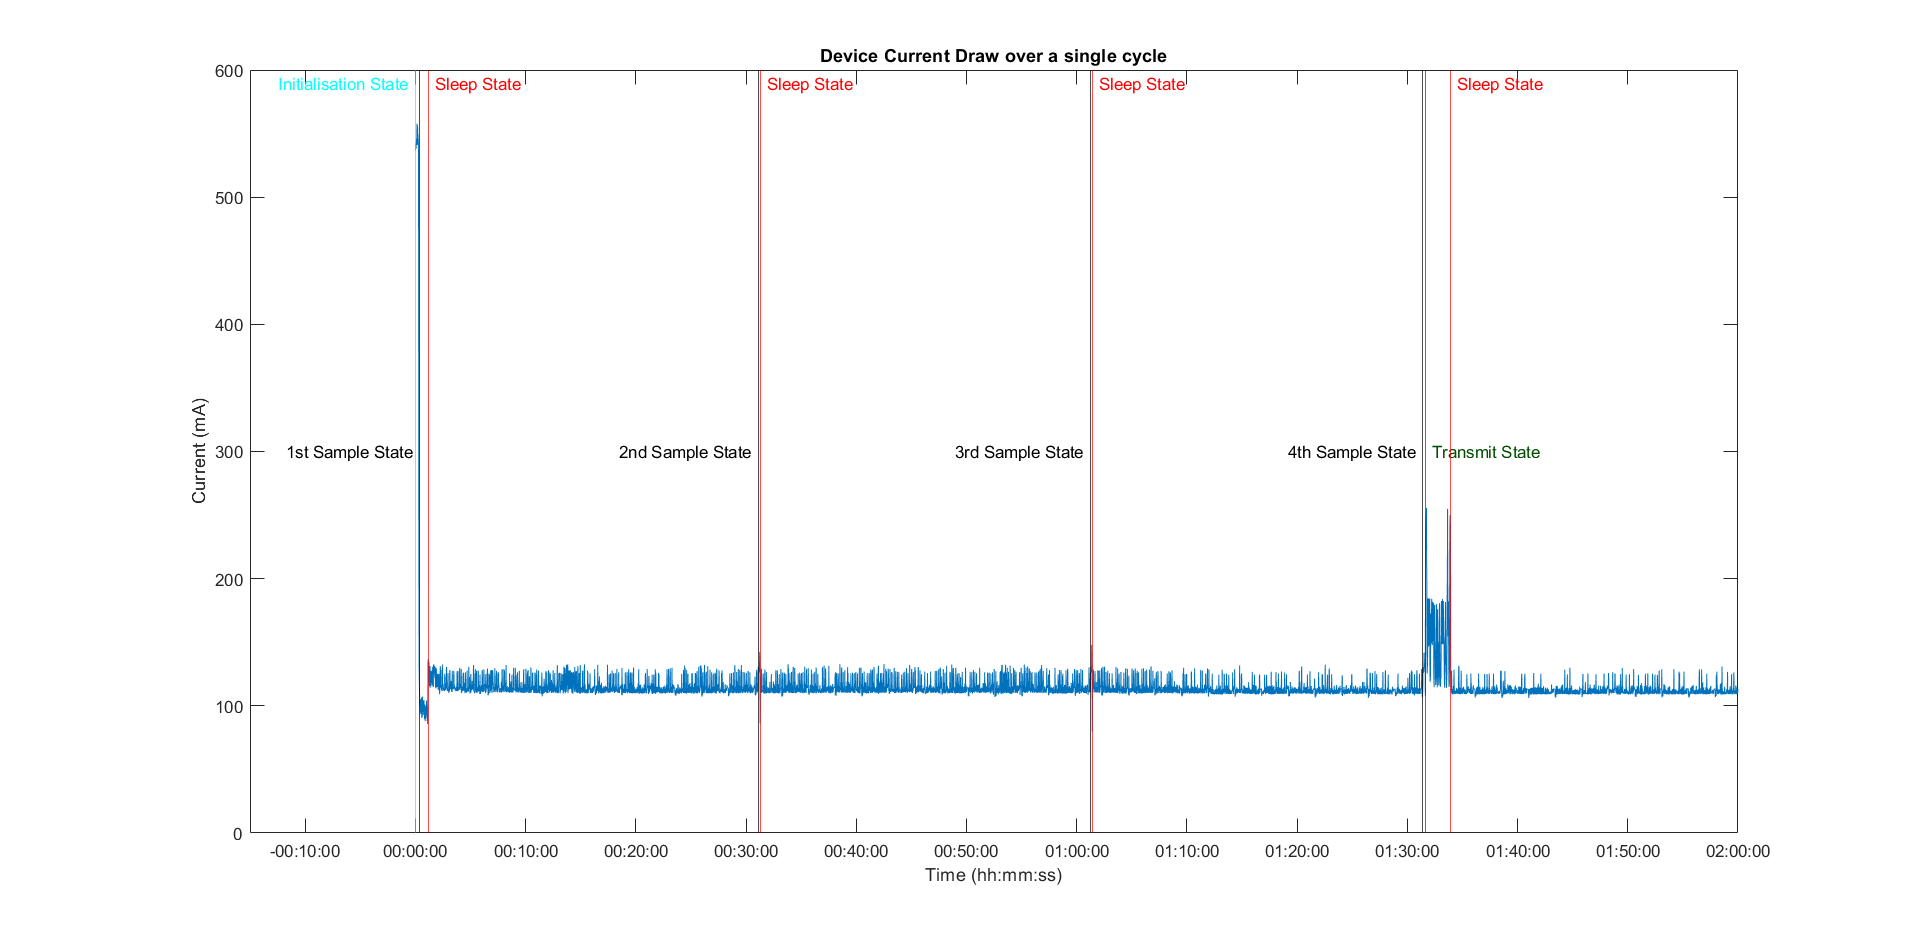
\includegraphics[width = \textwidth]{Power Cycle.png}
    \caption{Graph showing a typical current cycle of the buoy during the various phases. Data was sampled at 1Hz with all modules connected, sample intervals set to 30 mins the INA219 sensor connected to an external data logger and the device placed in a partially obstructed environment.}
    \label{fig:test_pwr_cycle}
\end{figure}


\begin{figure}[H]
    \centering
    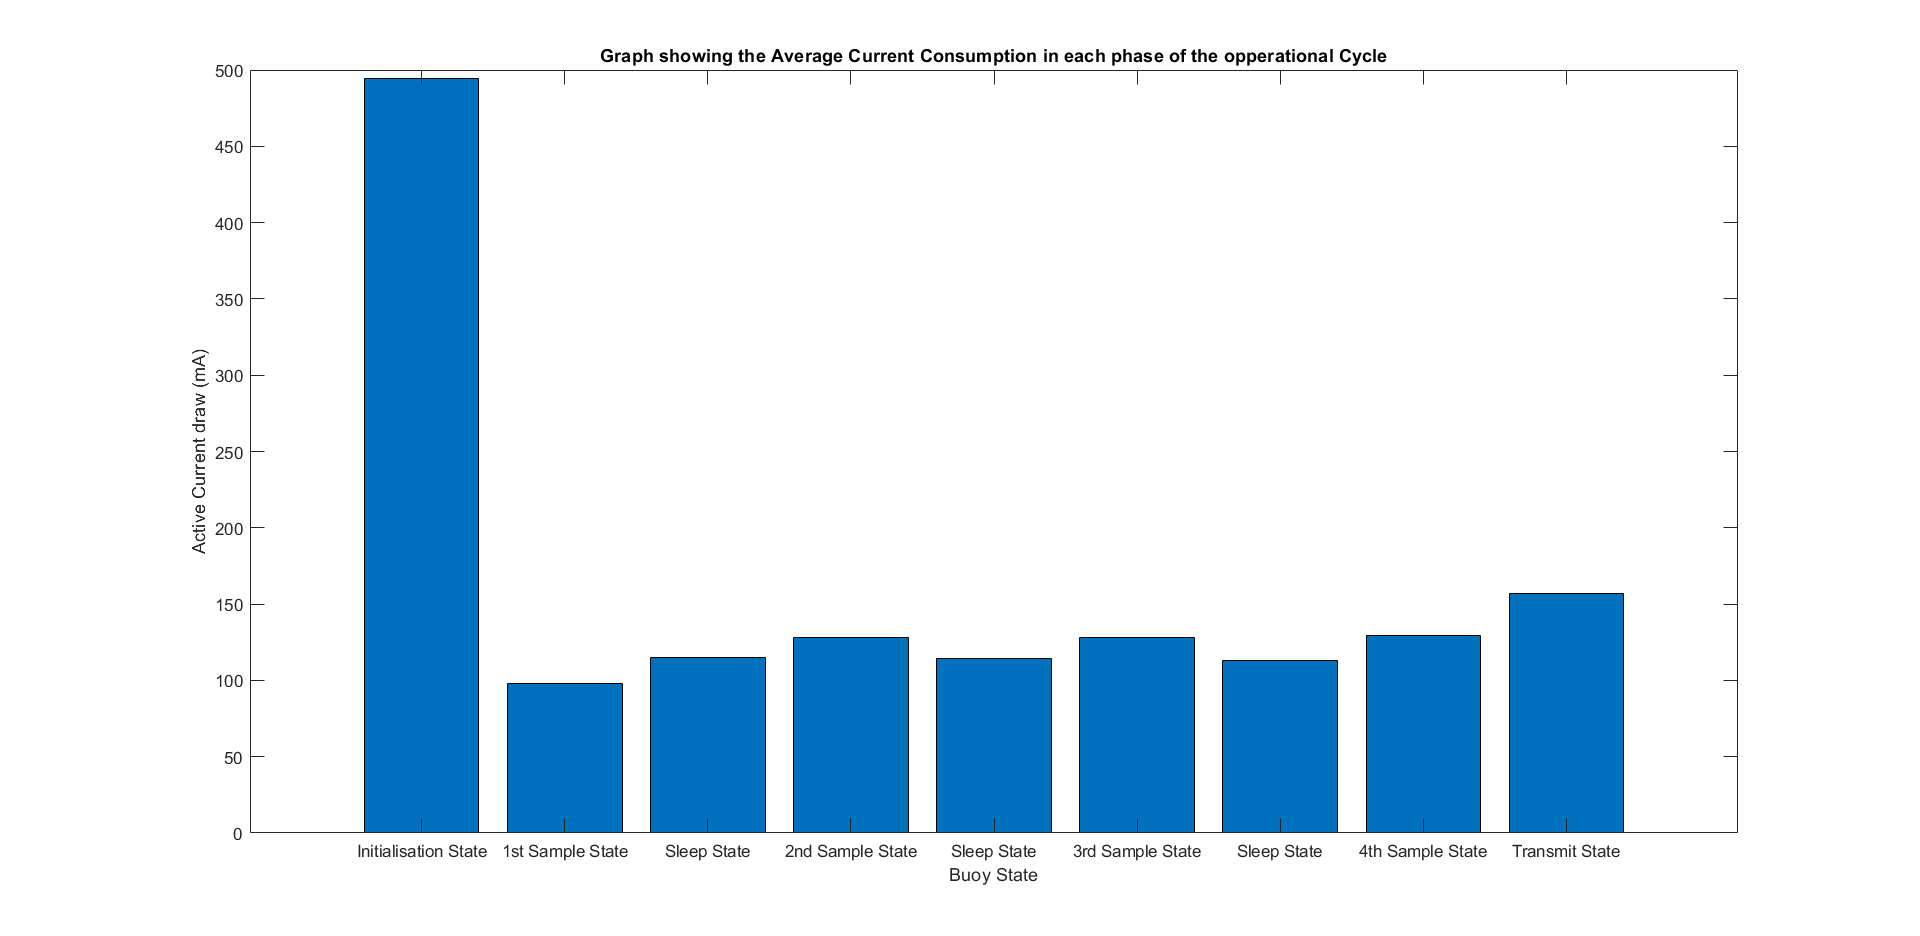
\includegraphics[width =\textwidth]{State Current Draw.png}
    \caption{Average Current consumption at each phase in the life-cycle of the buoy. Ordered chronologically}
    \label{fig:test_powtest_avgcurr}
\end{figure}

\begin{figure}[H]
    \centering
    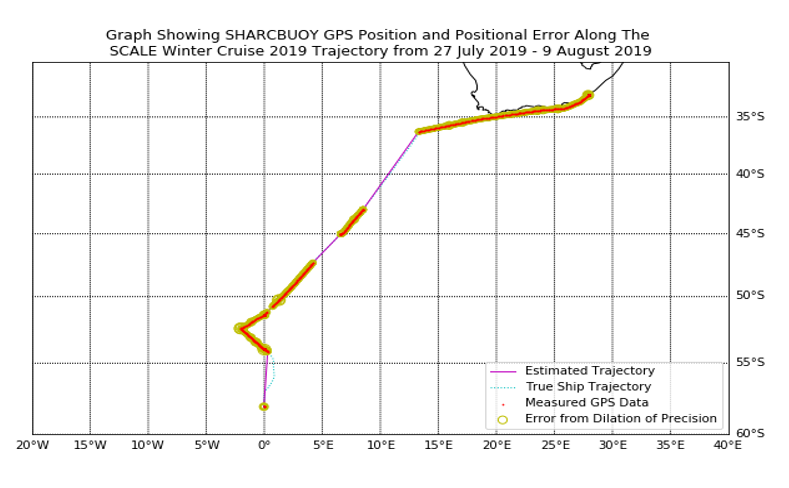
\includegraphics[scale=0.5]{gps_trajectory_scale2019.png}
    \caption{The GPS trajectory of the Aghulus 2 ship from the Marginal Ice Zone to East London. The plot shows the estimated position (magenta) taken from the buoy samples (red) compared to the actual trajectory (cyan). The positional error (PDOP) of each measurement is shown as an exaggerated area around the measured position}
    \label{fig:test_deploymenttest_GPS}
\end{figure}

\begin{figure}[H]
    \centering
    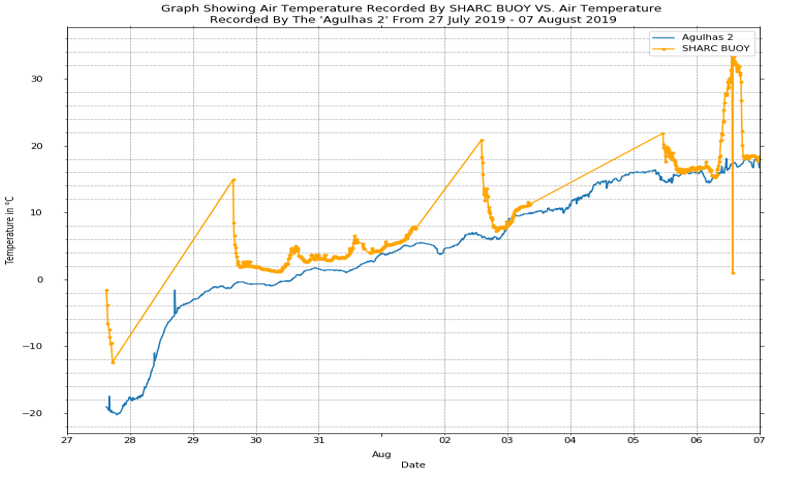
\includegraphics[scale=0.5]{temp_test_scale2019.png}
    \caption{Air Temperature recorded by the buoy (yellow) over 11 days compared to the air temperature recorded by the ship (blue) }
    \label{fig:test_deploymenttest_temp}
\end{figure}